Let $x_1(t)$ and $x_2(t)$ be two signals such that
\begin{align}
    y_1(t)&=tx_1(t)\\
    y_2(t)&=tx_2(t)
\end{align}
Figs. \ref{ec/2000/1/13/fig4}
 - \ref{ec/2000/1/13/fig4}
 show a graphical explanation.
\begin{figure}[!ht]
\centering
 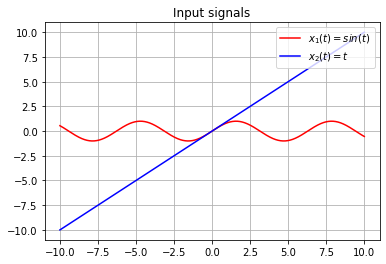
\includegraphics[width=\columnwidth]{solutions/ec/2000/1/13/figures/input signals.png}
 \caption{$x_1(t) = \sin{t}$ and $x_2(t) = t$}
 \label{ec/2000/1/13/fig1}
 \end{figure}
\begin{figure}[!ht]
\centering
 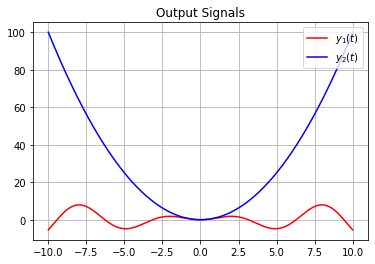
\includegraphics[width=\columnwidth]{solutions/ec/2000/1/13/figures/output signals.png}
 \caption{$y_1(t)$ and  $y_2(t)$}
 \end{figure}
 \begin{figure}[!ht]
\centering
 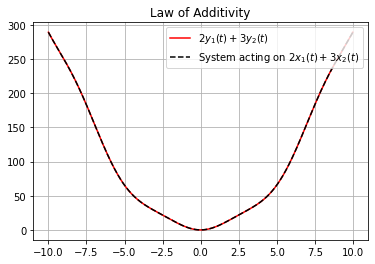
\includegraphics[width=\columnwidth]{solutions/ec/2000/1/13/figures/linear.png}
 \caption{The system obeys the law of superposition and hence is linear}
 \end{figure}
  \begin{figure}[!ht]
\centering
 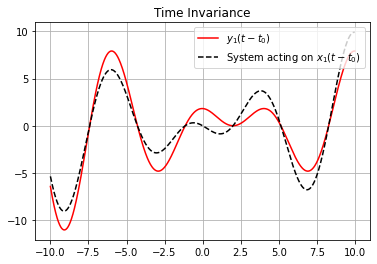
\includegraphics[width=\columnwidth]{solutions/ec/2000/1/13/figures/Time variant.png}
 \caption{Here delay in the input signal does not directly relate to a delay in the output signal. Hence, the system is not time invariant. }
 \label{ec/2000/1/13/fig4}
 \end{figure}
 Let
 \begin{align}
     x(t)&=\alpha x_1(t)+\beta x_2(t) \\
     y(t)&=tx(t)\\
     &=t(\alpha x_1(t)+\beta x_2(t))\\
     &=\alpha y_1(t) + \beta y_2(t)
 \end{align}
 Thus, the system is linear.
      Let there be a delay of $\delta$ in the input signal 
      \begin{align}
       x_{d}(t)&=x(t+\delta )  \\
       y(t)&=tx(t)\\
       y_{1}(t)&=tx_{d}(t)\\
       &=tx(t+\delta )
      \end{align}
     Now delay the output by $\delta$
 \begin{align}
  y(t)&=tx(t)\\
  y_{2}(t)&=y(t+\delta )\\
  &=(t+\delta )x(t+\delta )
 \end{align}
 Clearly $ y_{1}(t)\neq y_{2}(t)$, therefore the system is not time-invariant
 